\documentclass[11pt]{article}
\usepackage[utf8]{inputenc}
\usepackage[T1]{fontenc}
\usepackage{graphicx}
\usepackage[export]{adjustbox}
\graphicspath{ {./images/} }

\begin{document}
Normal Backwardation and Normal Contango

Backwardation and contango are typically discussed as the relationship between current spot prices and the prices of futures contracts of various settlement dates. This section discusses expected spot price and futures prices.

\section*{Normal Backwardation}
A somewhat subtle distinction exists between backwardation and normal backwardation. In normal backwardation, the forward price is believed to be below the expected spot price. We say "believed to be" because we cannot observe the expected spot price; we can only estimate it, and those estimations may differ between market participants. Since in normal backwardation the expected spot price exceeds the forward price, there is a positive expected return from holding the futures contract. Thus, a long position in a forward contract involves an expected profit in the case of normal backwardation (with no investment other than the posting of collateral that can earn interest).

Normal backwardation does not mean that markets are informationally inefficient, even though a forward contract in a market with normal backwardation would offer an expected profit with no investment; this is because any expected profit could be due to compensation for bearing risk. The concept of normal backwardation is silent on whether the expected profit of a long position is alpha or is a risk premium for bearing systematic risk. The entity on the long side of the forward contract should expect to earn a profit (a risk premium) for bearing the risk of being long the commodity whenever the underlying systematic risk (i.e., beta) is positive.

\section*{Normal Contango}
Normal contango is an infrequently used term that refers to the relationship between forward prices and expected spot prices in which the forward price is believed to be above the expected spot price. In normal contango, the entity on the short side of the forward contract should expect to earn a profit from bearing the risk of being short the commodity. Conversely, the entity on the long side of the forward contract should expect to bear a loss. In an informationally efficient market, normal contango would only exist for commodity forwards with negative betas (i.e., with returns that tend to hedge systematic risk). Since it would be relatively rare to expect a commodity to have negative beta, normal contango should be viewed as a rare occurrence. In an informationally inefficient market, normal contango would exist because a particular forward contract is overpriced and offers negative ex ante alpha to the long side and positive ex ante alpha to the short side.

\section*{Interpreting Normal Backwardation and Normal Contango}
Unlike backwardation and contango, normal backwardation and normal contango cannot be directly observed, because expected spot prices cannot be observed. It should be noted that the literature on commodities differs with regard to the distinction between backwardation and normal backwardation. The literature also differs about the distinction between contango and normal contango, and many sources do not even use the term normal contango. The definitions used in this session may not match the definitions that are found elsewhere, but they reflect the most consistent and useful definitions of the terms. The concepts involved are central to an organized understanding of the risks and returns of commodities and forward contracts on commodities, so it is necessary to use these terms with precision, even at the risk of having definitions that conflict with other sources.

Novices to forward markets sometimes assume that forward or futures prices are equal to expected spot prices. But in an efficient market, forward and futures prices must differ from expected spot prices whenever the position involves systematic risk. The excess of the expected spot price over the forward price is the expected reward for bearing the risk of being long the forward contract when the underlying asset has positive systematic risk. The expected loss to the short side of the contract is the cost of using the forward contract to hedge systematic risk. The only time that forward or futures prices should equal expected spot prices in an informationally efficient market is when the underlying asset contains no systematic risk.

In highly liquid futures markets such as the market for futures contracts on the S\&P 500, futures contracts are viewed as being cost-effective methods of obtaining exposure that is otherwise identical to a cash position in the S\&P 500. Unlike commodity futures, the components of the cost of carry on S\&P 500 futures contracts are somewhat easily observed (interest rates) or forecasted (dividend yields). Unlike some commodities, there are no harvests or inventory shortages for S\&P 500 exposure. Accordingly, issues such as the slope of the futures curve for S\&P 500 futures are largely ignored, since participants understand that the slope simply reflects the spread between interest rates and dividend yields. Also, decisions as to which S\&P 500 futures contracts to use (e.g., the nearby or deferred contracts) are based more on convenience and less on speculation with regard to changes in the basis.

In summary, in perfect capital markets, the price (or rates) of forward contracts on financial assets have term structures with slopes and curves that are driven entirely by the observable costs of carry (interest rates and distributions). In this case the relation between forward prices and expected spot prices is driven by risk premiums based on the systematic risks of the assets underlying the forwards. This understanding helps put the concepts of normal backwardation and normal contango in context: The relationship between expected spot prices and futures prices is not directly observable, it is determined by risk premiums, and it is distinct from the relation between current spot prices and current futures prices (which is determined by the costs of carry).

\section*{Keynes and Normal Backwardation}
John Maynard Keynes argued that commodity futures prices should typically be lower than the expected future spot prices (i.e., futures and forward markets should be in normal backwardation). Keynes's reasoning was based on the assumption that producers of a commodity have a strong incentive to lock in a sales price today for future production by selling futures contracts (artificially pushing down futures prices), but that users of the commodity have a strong incentive to purchase at spot prices (artificially raising spot pricing). If there is a natural oversupply of futures contracts, then speculators will enter the market to purchase the excess supply, but only at a discount to the expected future spot price. This exerts downward pressure on long-term futures prices relative to expected spot prices, leading to markets with normal backwardation.

In the fixed-income world, this argument is similar to the liquidity preference hypothesis. The liquidity preference hypothesis holds that producers of bonds (borrowers) prefer issuing long maturities, whereas consumers of bonds (lenders) prefer purchasing short maturities, distorting relative prices or rates from reflecting unbiased expectations. Producers offer attractive longer-term yields, which would mean relatively low long-term bond prices, to entice borrowers to extend their maturity or to induce speculators to borrow at short maturities and lend at long maturities. Thus, speculators are compensated for providing a service (time\\
intermediation) to the market. They provide demand by establishing long positions in long-term futures contracts to counter the excess supply generated by net short producers. This supports futures prices at a level above where they might lie in the absence of speculators. The positive risk premium entices speculators to enter the market despite the risk.

\section*{Commodity Forward Curves, Storage Costs, and Inventory Variation}
Models of a commodity forward curve predict that the curve will be upward sloping when the current inventory levels are much greater than the threshold levels of demand (low convenience yield), and that it will be downward sloping when inventories are exceptionally tight (high convenience yield). Storage models are unique to real assets. They do not have a corresponding model in fixed income because, except for financing, there is no cost of carry for bonds.

Another factor incorporated into storage models is the risk of stock-out, which occurs when storage effectively drops to zero, resulting in consumption being entirely dependent on production and transportation networks, and typically occurs in markets with peak seasonal demand, such as natural gas or heating oil, or with annual crop cycles, such as grains. To avoid stock-out, users of a commodity have an incentive to hedge more actively at points on the forward calendar that are most susceptible to stock-out. These would be the months just before harvest for annual crops, and the later part of the heating season for natural gas and heating oil.

The theory of storage a illustrated in the working curve, which positively relates the slope of the forward curve to current levels of inventory such that low inventory levels tend to be associated with a negative and nonlinear forward curve slope. The nonlinearity is due to embedded real options related to inventory levels. When inventory is low, users of the commodity may face costs related to searching, delays, rush charges, and transportation. In the extreme, they may face significant costs from stock-outs as inventory is depleted.

\section*{Commodity Forward Prices and the Market Segmentation Hypothesis}
The section entitled Keynes and Normal Backwardation discusses the possibility that commodity forward curves are determined by a liquidity preference or liquidity premium and the desire of producers to hedge their anticipated commodity sales with short positions in long-term forwards or futures. In some markets, the users of a commodity rarely use the forward market to hedge future commodity needs. These particular markets typically exist for products that are directly consumed by the public, such as gasoline.

In some cases, the forward curve may be better explained by the reasoning used in fixed-income markets in discussions of the market segmentation (i.e., preferred habitat) hypothesis, in which the relation between expected spot rates and forward rates varies nonmonotonically throughout the range of delivery dates due to supply and demand pressures in localized regions of the curve.

Under the market segmentation hypothesis, the net supply or demand for specific futures contracts by natural hedgers could be positive or negative depending on market conditions and preferences of producers and users to hedge their risks. As a result, speculators may need to take short or long positions to absorb the excess demand or the excess supply of futures contracts created by hedgers. To the extent that market participants demand substantial risk premiums to stray from using their preferred time to settlement to another longevity, the risk premium in the futures markets could vary across times to settlement. In other words, if participants have a preferred habitat (i.e., time to settlement) and the market is segmented (participants are reluctant to hedge contracts of varying times to settlement), there could be nonmonotonic slopes to forward curves, such as a humped curve.

The crude oil futures market has often exhibited a humped curve, which in the typical case of commodity futures means that the market is in contango in the short term, but gives way to backwardation for longer-maturity contracts. The exhibit below depicts a humped curve.

\begin{center}
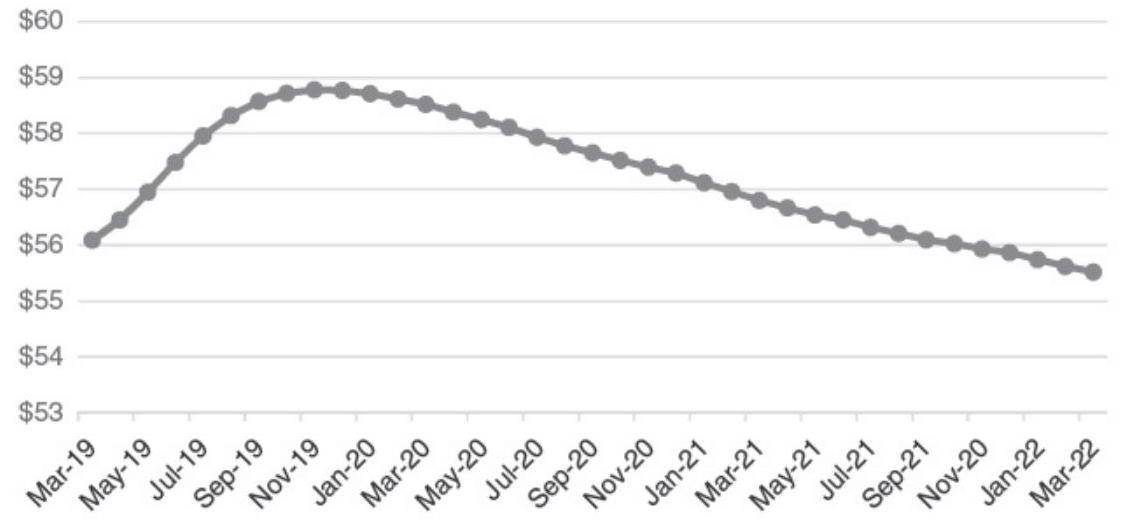
\includegraphics[max width=\textwidth]{2024_04_11_0af5e5bdb875454d1acag-3}
\end{center}

\section*{Crude Oil Futures Curve}
\section*{Option-Based Models of the Forward Curve for Commodities}
Option-based models of the term structure focus on two types of real options embedded in commodity markets. Real options embedded in commodity markets are implied options involving real assets.

The first type of real option is the option to extract a natural resource. A copper mine can be shut down if the price of copper falls below the marginal cost of production. Although there may be times when the spot price of copper falls below its marginal cost of production due to a temporary glut, producers will not sell forward production below cost for long; that is, they will shut down the mine. The option to extract (or defer extraction of) the resource dampens the volatility of commodity prices for future delivery.

The second real option embedded in the commodity forward curve is related to inventories. Commodity markets generally have a volatility asymmetry. A volatility asymmetry is a difference in values between two analogous volatilities, such as is the case with commodities, in which volatility tends to be higher when prices are\\
rising than when they are falling. This is because shortages tend to cause more serious problems than surpluses. The volatility asymmetry favors owning physical inventory (or short-dated futures contracts) over longer-dated futures contracts. All other things being equal, this factor will tend to flatten commodity futures curves or lead to backwardation.


\end{document}